\chapter{Notation and Definition}

\section{Notation}

We will review all the necessary notation and mathematics for us to continue the journey of Machine Learning.

\subsection{Data Structure}

A \textbf{scalar} is simple numerical value, like $15$ or $-3.25$, denoted by an italic letter, like $x$ or $a$. A \textbf{vector} is an ordered list of scalar values, called attributes. Vector is denoted by bold character $\mathbf{x}$ or $\mathbf{w}$. A \textbf{matrix} is a rectangular array of numbers arranged in rows and columns.

\begin{figure}[H]
	\begin{subfigure}[t]{0.45\linewidth}
		\centering
		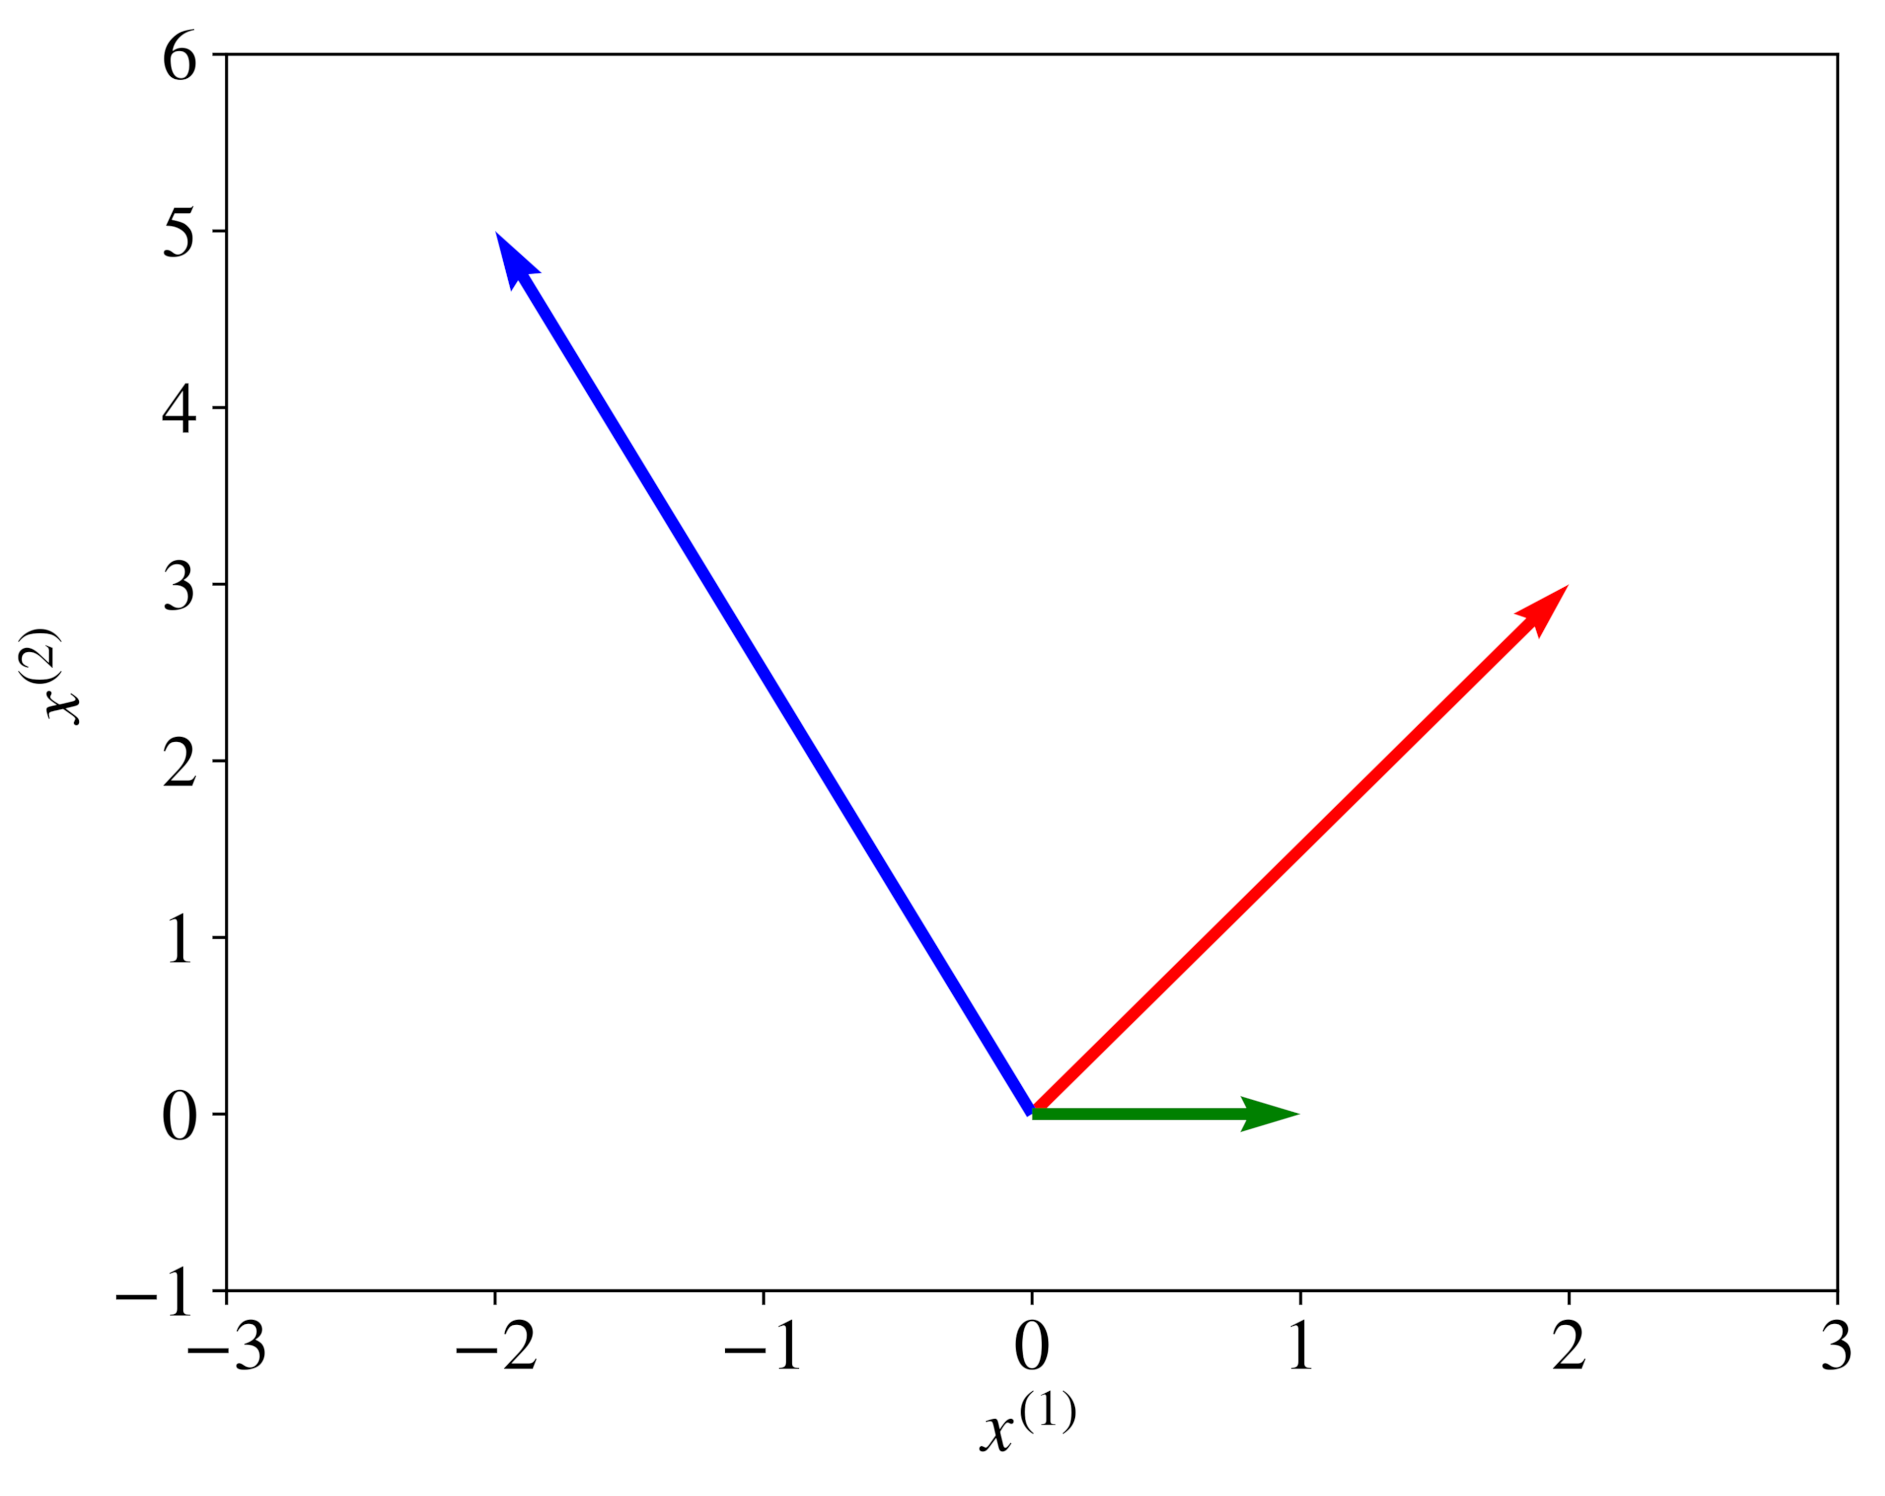
\includegraphics[width=\linewidth]{imgs/notation/notation_1}
		\caption{First subfigure}
	\end{subfigure}
	\hfill % this will put some space between your two figures
	\begin{subfigure}[t]{0.45\linewidth}
		\centering
		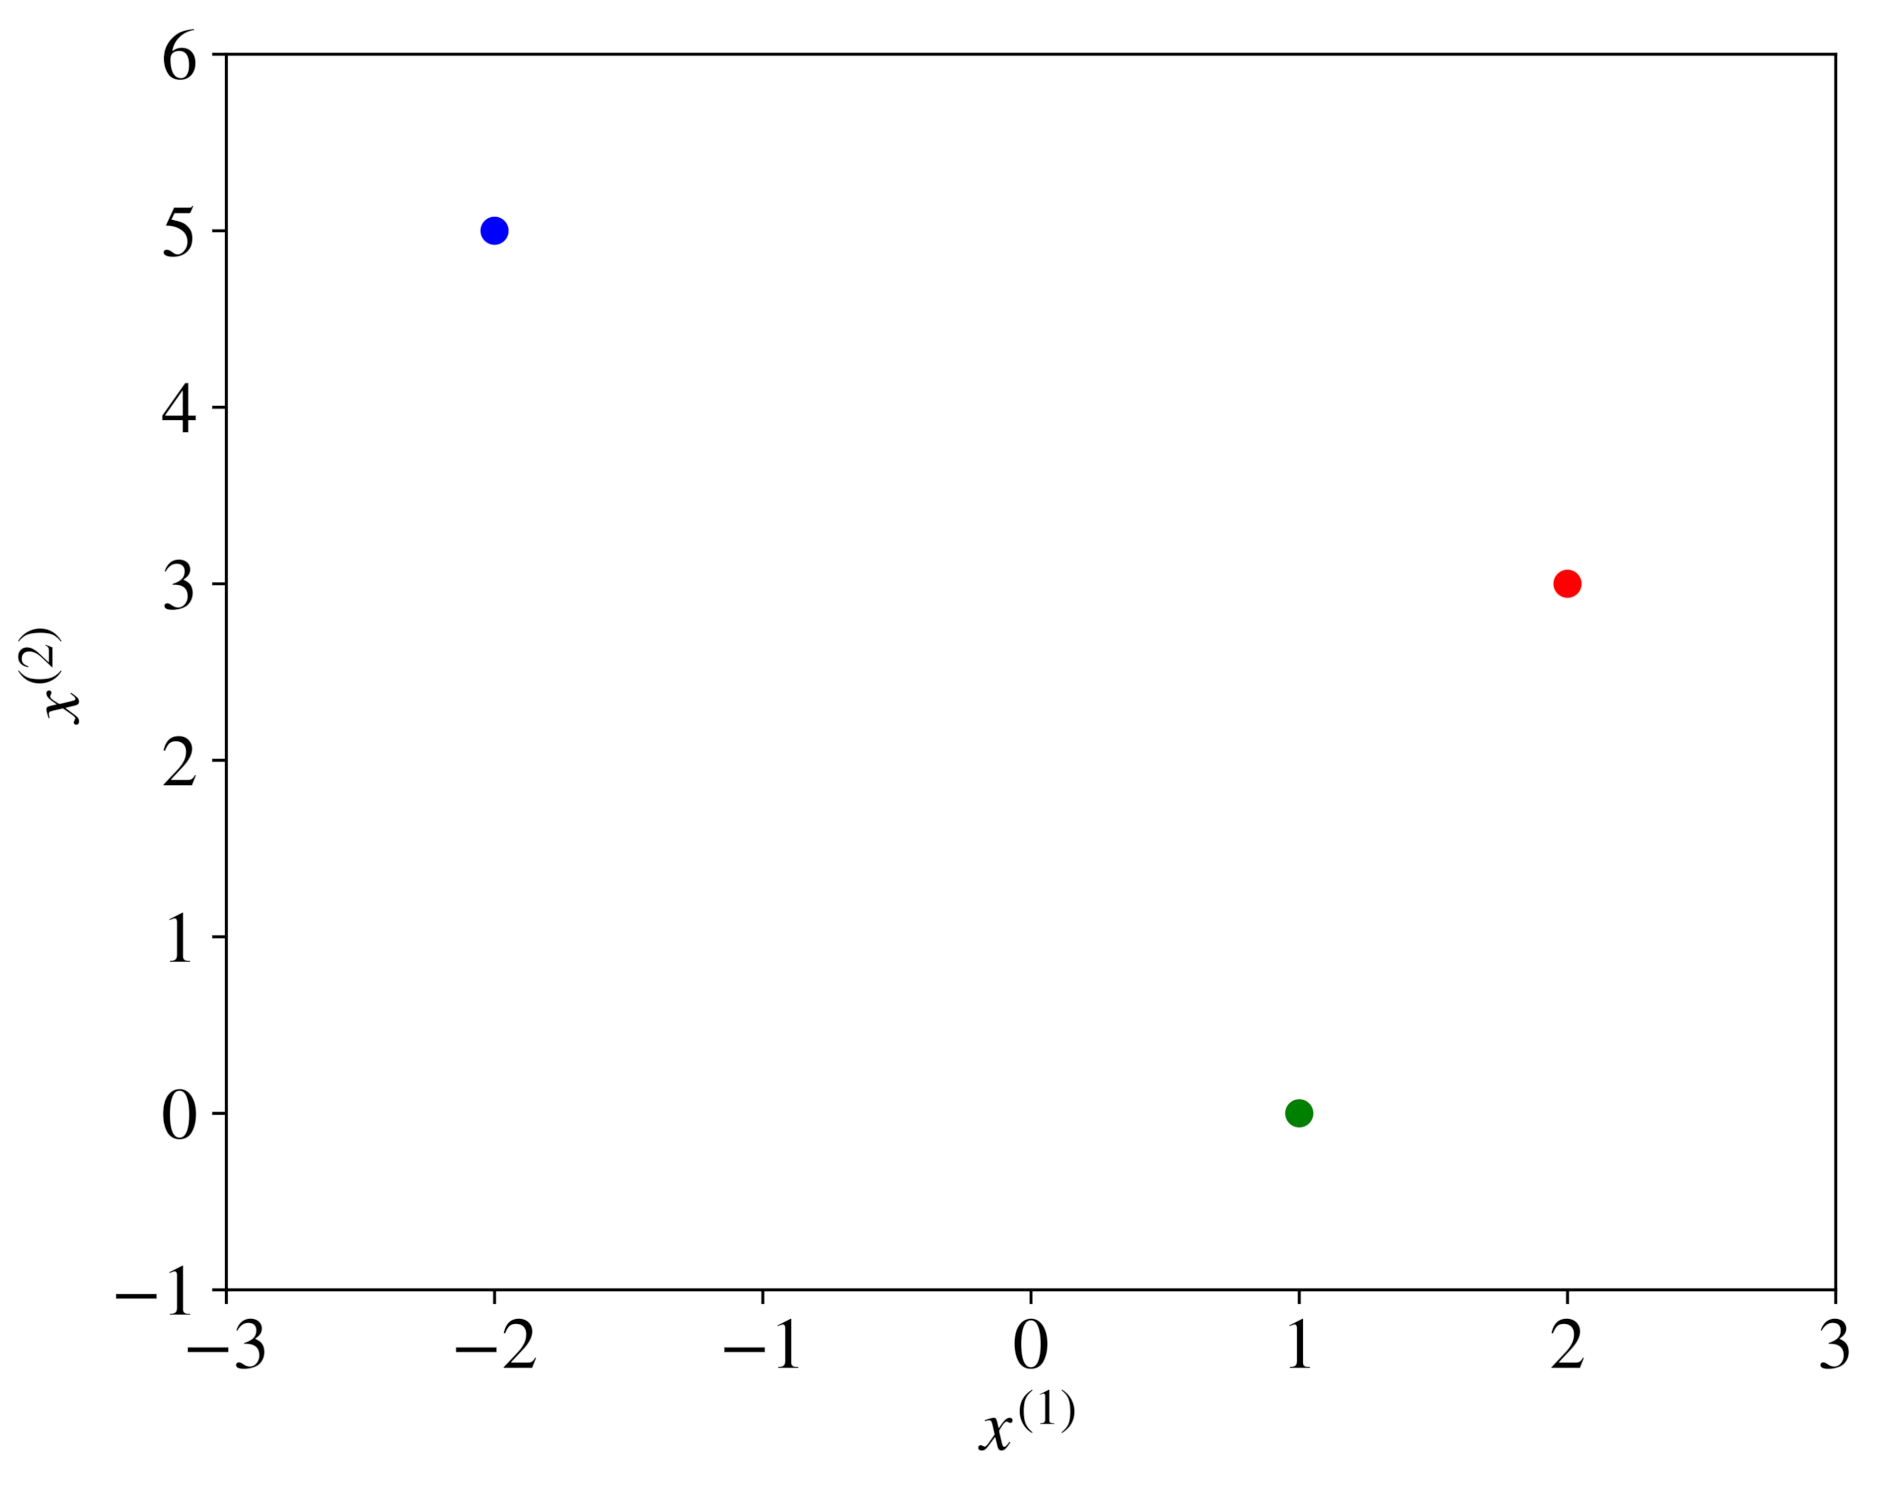
\includegraphics[width=\linewidth]{imgs/notation/notation_2}
		\caption{Second subfigure}
	\end{subfigure}
	\caption{Three vectors visualized as directions and as points.}
	\label{fig:notation_1}
\end{figure}

A \textbf{matrix} is a rectangular array of numbers arranged in rows and columns, which are denoted with bold capital letters, such as $\mathbf{A}$ or $\mathbf{W}$.  A \textbf{set} is an unordered collection of unique elements. We denote a set as a calligraphic capital character, for example, \(\mathcal{S}\). When an element belongs to a set \(\mathcal{S}\) , we write $x\in\mathcal{S}$. We can obtain a new set $\mathcal{S}_3$ as an \textbf{intersection} of two set $\mathcal{S}_1$ and $\mathcal{S}_2$, written as $\mathcal{S} \leftarrow\mathcal{S}_{1} \cap \mathcal{S}_{2}$. Also we can obtain a new set by \textbf{union}, $\mathcal{S}_3\leftarrow\mathcal{S}_1\cup\mathcal{S}_2$.

\subsection{Capital Sigma Notation}
The summation over a collection \(\mathcal{X}=\left\{x_{1}, x_{2}, \ldots, x_{n-1}, x_{n}\right\}\) or over the attributes of a vector $\mathbf{x}=\left[x^{(1)}, x^{(2)}, \ldots, x^{(m-1)}, x^{(m)}\right]$ is denoted like this:
\begin{equation*}
	\sum_{i=1}^{n} x_{i} \stackrel{\text { def }}{=} x_{1}+x_{2}+\ldots+x_{n-1}+x_{n}, \text { or else: } \sum_{j=1}^{m} x^{(j)} \stackrel{\text { def }}{=} x^{(1)}+x^{(2)}+\ldots+x^{(m-1)}+x^{(m)}
\end{equation*}
The notation $\stackrel{\text { def }}{=}$ means ``is defined as".

\subsection{Capital Pi Notation}

\begin{equation*}
	\prod_{i=1}^{n} x_{i} \stackrel{\text { def }}{=} x_{1} \cdot x_{2} \cdot \ldots \cdot x_{n-1} \cdot x_{n}
\end{equation*}
\begin{itemize}
	\item A product of elements in a collection or attributes of a vector.
\end{itemize}

\subsection{Operations on Sets}

Given the expression:
\[ \mathcal{S}^{\prime} \leftarrow \left\{x^{2} \mid x \in \mathcal{S}, x > 3\right\} \]
This notation is used to define a derived set creation operator. It means that we create a new set \( \mathcal{S}^{\prime} \) by including the square of each element \( x \) from the set \( \mathcal{S} \), under the condition that \( x \) is greater than 3. In other words, \( \mathcal{S}^{\prime} \) is comprised of the squares of all elements in \( \mathcal{S} \) which are greater than 3.

Additionally, the cardinality operator \( |\mathcal{S}| \) is used to denote the number of elements in the set \( \mathcal{S} \). For example, if \( \mathcal{S} = \{1, 2, 4, 5\} \), then \( \mathcal{S}^{\prime} = \{16, 25\} \) as only 4 and 5 from \( \mathcal{S} \) satisfy the condition \( x > 3 \). The \textbf{cardinality} \( |\mathcal{S}| \) in this case would be 4.

\subsection{Operations on Vectors}

\textbf{Vector Addition and Subtraction:}
The sum and difference of two vectors \( \mathbf{x} \) and \( \mathbf{z} \) are defined component-wise as:
\[ \mathbf{x} + \mathbf{z} = \left[x^{(1)} + z^{(1)}, \ldots, x^{(m)} + z^{(m)}\right] \]
\[ \mathbf{x} - \mathbf{z} = \left[x^{(1)} - z^{(1)}, \ldots, x^{(m)} - z^{(m)}\right] \]
\emph{Example:} For \( \mathbf{x} = [1, 2] \) and \( \mathbf{z} = [3, 4] \),
\[ \mathbf{x} + \mathbf{z} = [1+3, 2+4] = [4, 6] \]

\textbf{Scalar Multiplication:}
A vector multiplied by a scalar \( c \) results in a scaled vector:
\[ \mathbf{x} c = \left[c x^{(1)}, \ldots, c x^{(m)}\right] \]
\emph{Example:} For \( \mathbf{x} = [1, 2] \) and \( c = 3 \),
\[ \mathbf{x} c = [3 \times 1, 3 \times 2] = [3, 6] \]

\textbf{Dot Product:}
The dot product of two vectors \( \mathbf{w} \) and \( \mathbf{x} \) is a scalar:
\[ \mathbf{w} \mathbf{x} = \sum_{i=1}^{m} w^{(i)} x^{(i)} \]
\emph{Example:} For \( \mathbf{w} = [1, 2] \) and \( \mathbf{x} = [3, 4] \),
\[ \mathbf{w} \mathbf{x} = 1 \times 3 + 2 \times 4 = 3 + 8 = 11 \]
\textbf{Matrix-Vector Multiplication:}
Multiplying a matrix \( \mathbf{W} \) by a vector \( \mathbf{x} \) yields another vector. For example:
$$
	\begin{aligned}
		\mathbf{W} \mathbf{x} & =\left[\begin{array}{lll}
				                               w^{(1,1)} & w^{(1,2)} & w^{(1,3)} \\
				                               w^{(2,1)} & w^{(2,2)} & w^{(2,3)}
			                               \end{array}\right]\left[\begin{array}{l}
				                                                       x^{(1)} \\
				                                                       x^{(2)} \\
				                                                       x^{(3)}
			                                                       \end{array}\right]                                      \\
		                      & \stackrel{\text { def }}{=}\left[\begin{array}{l}
				                                                         w^{(1,1)} x^{(1)}+w^{(1,2)} x^{(2)}+w^{(1,3)} x^{(3)} \\
				                                                         w^{(2,1)} x^{(1)}+w^{(2,2)} x^{(2)}+w^{(2,3)} x^{(3)}
			                                                         \end{array}\right] \\
		                      & =\left[\begin{array}{l}
				                               \mathbf{w}^{(1)} \mathbf{x} \\
				                               \mathbf{w}^{(2)} \mathbf{x}
			                               \end{array}\right]
	\end{aligned}
$$

\emph{Example:} For
\[ \mathbf{W} = \left[\begin{array}{ll}
			1 & 2 \\
			3 & 4
		\end{array}\right] \text{ and } \mathbf{x} = \left[\begin{array}{l}
			5 \\
			6
		\end{array}\right], \]
\[ \mathbf{W} \mathbf{x} = \left[\begin{array}{l}
			1 \times 5 + 2 \times 6 \\
			3 \times 5 + 4 \times 6
		\end{array}\right] = \left[\begin{array}{l}
			17 \\
			39
		\end{array}\right] \]
\textbf{Transpose and Multiplication:}
For the transpose of a vector \( \mathbf{x} \) denoted \( \mathbf{x}^{\top} \), and a matrix \( \mathbf{W} \), the multiplication \( \mathbf{x}^{\top} \mathbf{W} \) is given by:
$$
	\begin{aligned}
		\mathbf{x}^{\top} \mathbf{W} & =\left[\begin{array}{ll}
				                                      x^{(1)} & x^{(2)}
			                                      \end{array}\right]\left[\begin{array}{lll}
				                                                              w^{(1,1)} & w^{(1,2)} & w^{(1,3)} \\
				                                                              w^{(2,1)} & w^{(2,2)} & w^{(2,3)}
			                                                              \end{array}\right]                                                                                      \\
		                             & \stackrel{\text { def }}{=}\left[w^{(1,1)} x^{(1)}+w^{(2,1)} x^{(2)}, w^{(1,2)} x^{(1)}+w^{(2,2)} x^{(2)}, w^{(1,3)} x^{(1)}+w^{(2,3)} x^{(2)}\right]
	\end{aligned}
$$

\emph{Example:} For
\[ \mathbf{x} = \left[\begin{array}{l}
			7 \\
			8
		\end{array}\right] \text{ and } \mathbf{W} = \left[\begin{array}{lll}
			1 & 2 & 3 \\
			4 & 5 & 6
		\end{array}\right], \]
\[ \mathbf{x}^{\top} \mathbf{W} = \left[\begin{array}{lll}
			7 \times 1 + 8 \times 4, 7 \times 2 + 8 \times 5, 7 \times 3 + 8 \times 6
		\end{array}\right] = \left[\begin{array}{lll}
			39, 54, 69
		\end{array}\right] \]

\subsection{Functions}

\textbf{Definition of a Function}\\
A function is a relation that associates each element \( x \) of a set \( \mathcal{X} \), known as the domain, to a single element \( y \) of another set \( \mathcal{Y} \), known as the codomain. This relation is denoted as \( y = f(x) \), where \( f \) is the name of the function, \( x \) is the input or argument, and \( y \) is the output. The input variable is also referred to as the variable of the function.

\emph{Example:} Consider the function \( f(x) = x^2 \) defined on the domain \( \mathcal{X} = \mathbb{R} \). For \( x = 2 \), the output is \( f(2) = 2^2 = 4 \).

\textbf{Local and Global Minima}\\
The function \( f(x) \) has a local minimum at \( x = c \) if \( f(x) \geq f(c) \) for every \( x \) in an open interval around \( c \). An open interval, such as \( (0,1) \), includes all numbers between its endpoints but not the endpoints themselves. The smallest value among all local minima is known as the global minimum.

\emph{Example:} In the function \( f(x) = (x-1)^2 \), the local (and global) minimum occurs at \( x = 1 \) since \( f(x) \geq f(1) = 0 \) for all \( x \).

\begin{figure}[H]
	\centering
	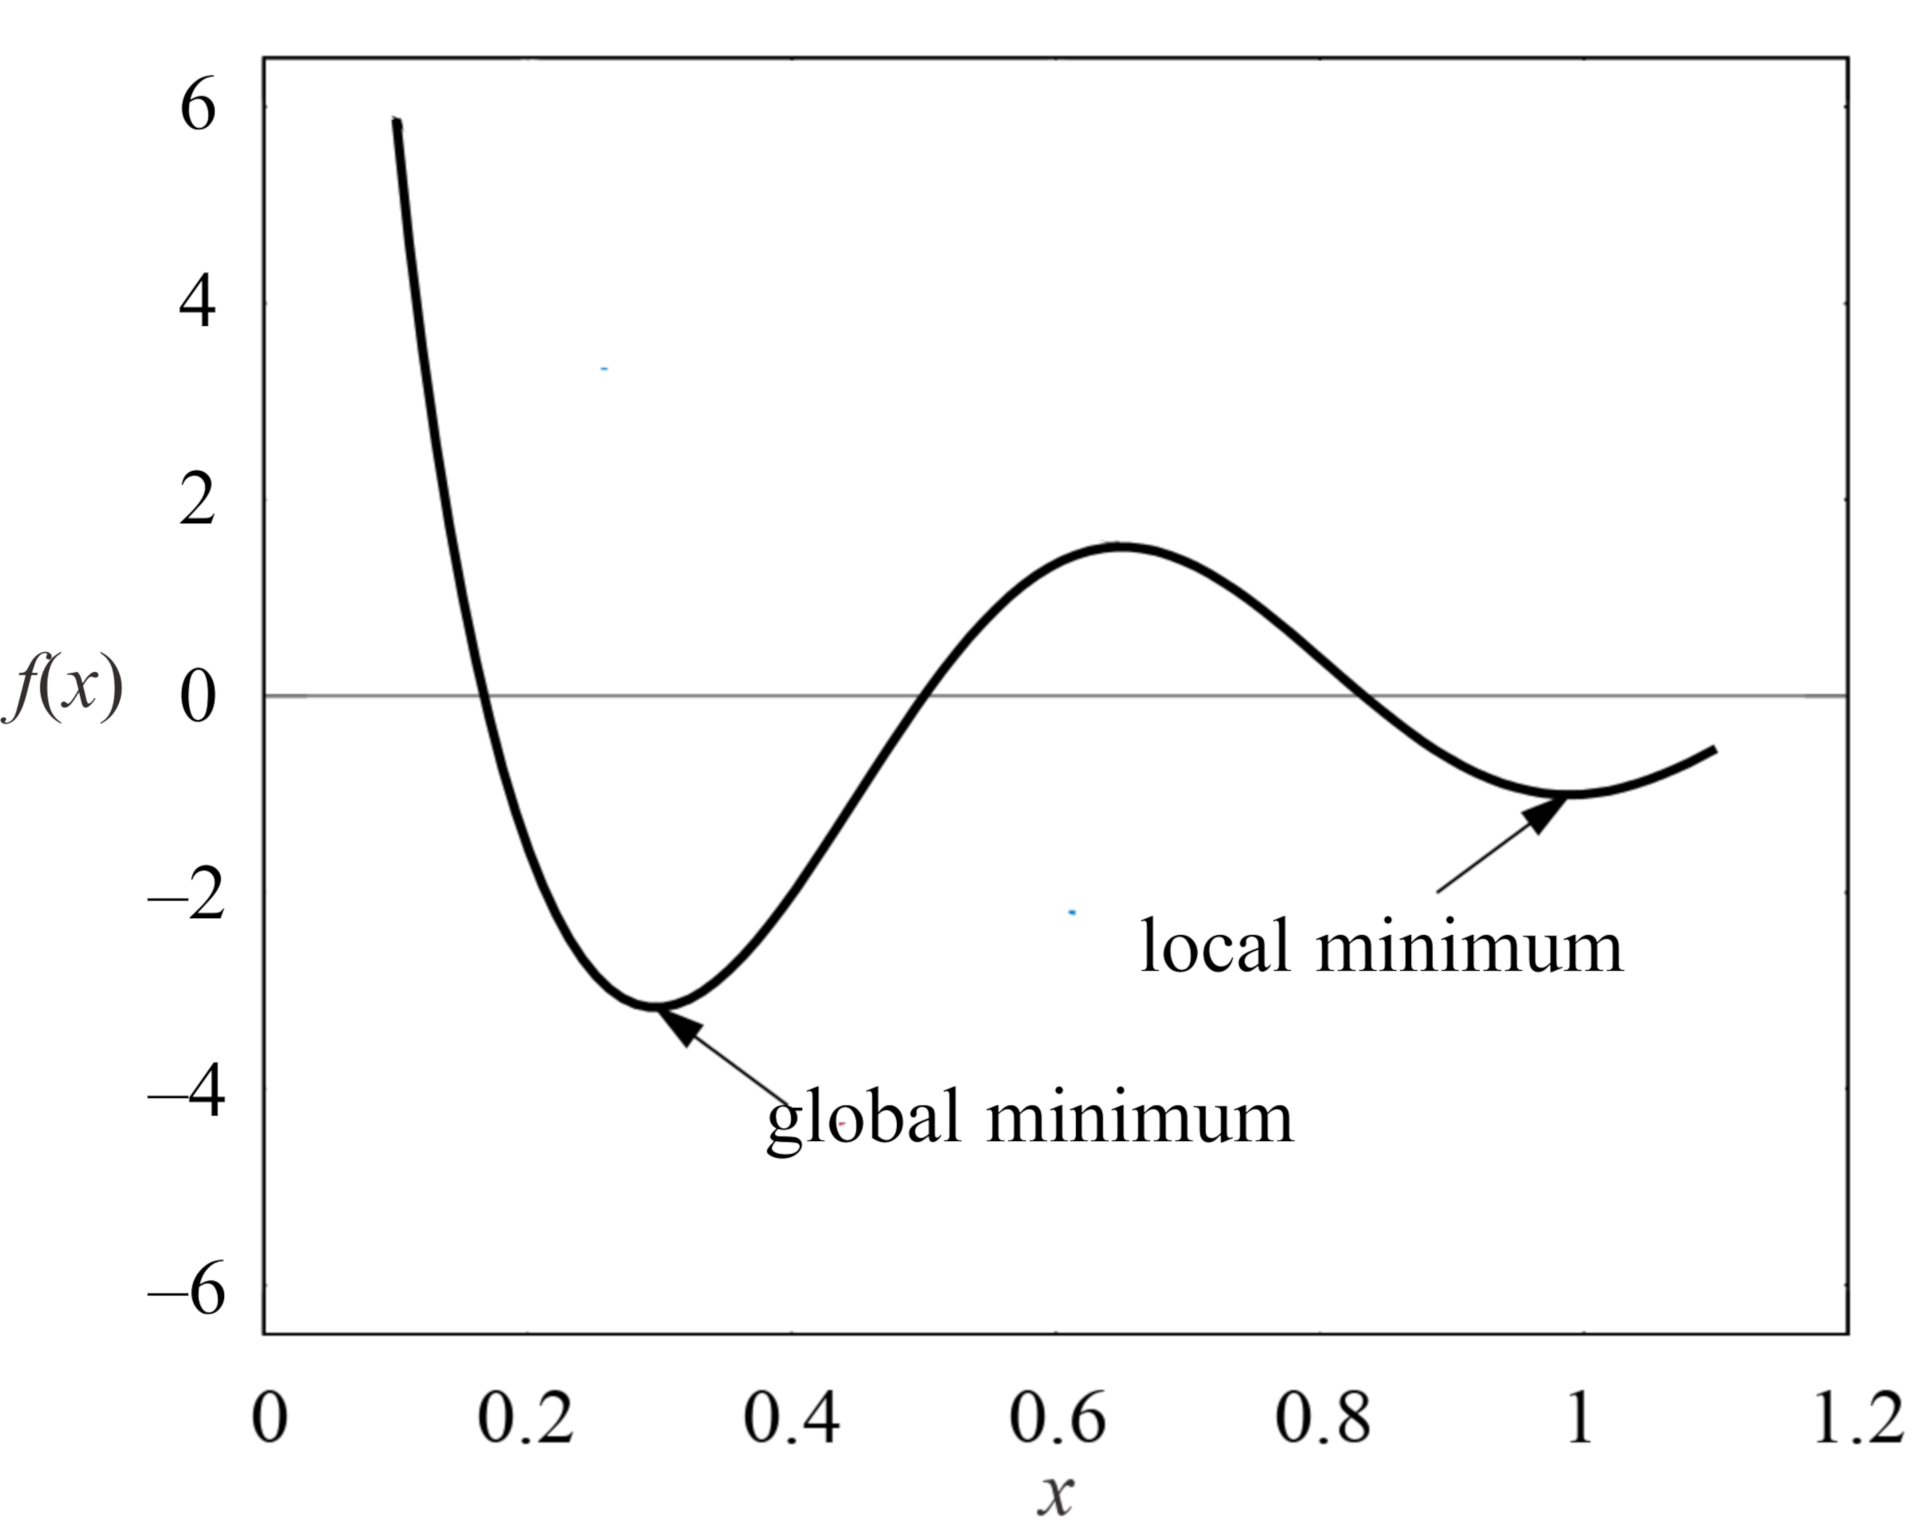
\includegraphics[width=0.7\linewidth]{imgs/notation/notation_3.png}
	\caption{A local and a global minima of a function.}
	\label{fig:notation_3}
\end{figure}

\textbf{Vector Functions}\\
A vector function, denoted \( \mathbf{y} = \mathbf{f}(x) \), is a function that returns a vector \( \mathbf{y} \). Its argument can be either a vector or a scalar.

\emph{Example:} For the vector function \( \mathbf{f}(x) = [x, x^2] \), with \( x = 2 \), the output is \( \mathbf{f}(2) = [2, 2^2] = [2, 4] \).

\subsection{Max and Arg Max}

Given a set of values \( \mathcal{A} = \{a_{1}, a_{2}, \ldots, a_{n}\} \), the operator \( \max_{a \in \mathcal{A}} f(a) \) returns the highest value of \( f(a) \) for all elements in the set \( \mathcal{A} \). Conversely, the operator \( \arg \max_{a \in \mathcal{A}} f(a) \) identifies the specific element \( a \) in the set \( \mathcal{A} \) that maximizes the function \( f(a) \).

In cases where the set is implicit or infinite, we can use the notation \( \max_{a} f(a) \) or \( \arg \max_{a} f(a) \) respectively. Similarly, the operators \( \min \) and \( \arg \min \) function in a comparable way, determining the lowest value of a function and the

\subsection{Assignment Operator}
The expression \(a \leftarrow f(x)\) means that the variable \(a\) gets the new value: the result of \(f(x)\). We say that the variable \(a\) gets assigned a new value. Similarly, \(\mathbf{a} \leftarrow\left[a_{1}, a_{2}\right]\) means that the vector variable \(\mathbf{a}\) gets the two-dimensional vector \(\left[a_{1}, a_{2}\right]\).

\subsection{Derivative and Gradient}
A \textbf{derivative} \(f^{\prime}\) of a function \(f\) is a function or a value that describes how fast \(f\) grows (or decreases). If the derivative \(f^{\prime}\) is a function, then the function \(f\) can grow at a different pace in different regions of its domain.

we can use \textbf{chain rule} when we encounter hard-to-differentiate function. For instance if \(F(x)=f(g(x))\), where \(f\) and \(g\) are some functions, then \(F^{\prime}(x)= f^{\prime}(g(x)) g^{\prime}(x)\).

\textbf{Gradient} is the generalization of derivative for functions that take several inputs (or one input in the form of a vector or some other complex structure). A gradient of a function is a vector of \textbf{partial derivatives}. For example, \(f\left(\left[x^{(1)}, x^{(2)}\right]\right)=a x^{(1)}+b x^{(2)}+c\), then the partial derivative of function \(f\) \textit{with respect to} \(x^{(1)}\), denoted as \(\frac{\partial f}{\partial x^{(1)}}\), is given by,
$$
	\frac{\partial f}{\partial x^{(1)}}=a+0+0=a
$$
where \(a\) is the derivative of the function \(a x^{(1)}\); the two zeroes are respectively derivatives of
\(b x^{(2)}\) and \(c\), because \(x^{(2)}\) is considered constant when we compute the derivative with respect
to \(x^{(1)}\), and the derivative of any constant is zero. Similarly, the partial derivative of function \(f\) with respect to \(x^{(2)}, \frac{\partial f}{\partial x^{(2)}}\), is given by,
$$
	\frac{\partial f}{\partial x^{(2)}}=0+b+0=b
$$

The gradient of function \(f\), denoted as \(\nabla f\) is given by the vector \(\left[\frac{\partial f}{\partial x^{(1)}}, \frac{\partial f}{\partial x^{(2)}}\right]\).

\section{Random Variable}

A \textbf{random variable}, usually written as an italic letter, like \(X\), is a variable whose possible values are numerical outcomes of a random phenomenon. There are two types of random variables: \textbf{discrete} and \textbf{continuous}. A \textbf{discrete random variable} takes on only countable number of distinct values such as \textit{red}, \textit{yellow}, \textit{blue} or 1,2,3, . . ..

\begin{figure}[H]
	\centering
	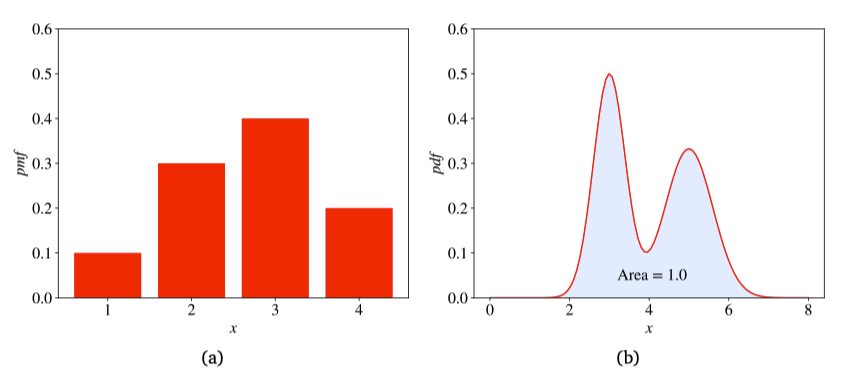
\includegraphics[width=0.7\linewidth]{imgs/notation/notation_4.png}
	\caption{A probability mass function and a probability density function.}
	\label{fig:notation_4}
\end{figure}
The \textbf{probability distribution} of a discrete random variable is described by a list of probability associated with each of its possible values. This list of probability is called a \textbf{probability mass function} (pmf)(Fig.\ref{fig:notation_4}, \textbf{a}).

A \textbf{continuous random variable} takes an infinite number of possible values in some interval. The probability distribution of a continual random variable (a continuous probability distribution) is described by a \textbf{probability density function} (pdf) (Fig.\ref{fig:notation_4}, \textbf{b}).

Let a discrete random variable \(X\) have \(k\) possible values \(\left\{x_{i}\right\}_{i=1}^{k}\). The \textbf{expectation} of \(X\) denoted as \(\mathbb{E}[X]\) is given by,

\begin{equation}
		\begin{aligned}
			 \mathbb{E}[X] & \stackrel{\text { def }}{=} \sum_{i=1}^{k}\left[x_{i} \cdot \operatorname{Pr}\left(X=x_{i}\right)\right] \\ & =x_{1} \cdot \operatorname{Pr}\left(X=x_{1}\right)+x_{2} \cdot \operatorname{Pr}\left(X=x_{2}\right)+\cdots+x_{k} \cdot \operatorname{Pr}\left(X=x_{k}\right)
		\end{aligned}
		\label{notation:1}
\end{equation}

where \(\operatorname{Pr}\left(X=x_{i}\right)\) is the probability that \(X\) has the value \(x_{i}\) according to the pmf. The expectation of a random variable is also called the \textbf{mean}, \textbf{average} or \textbf{expected value} and is frequently denoted with the letter \(\mu\),

Now the \textbf{standard deviation}, defined as,
$$
	\sigma \stackrel{\text { def }}{=} \sqrt{\mathbb{E}\left[(X-\mu)^{2}\right]}
$$
\textbf{Variance}, denoted as \(\sigma^{2}\) or \(\operatorname{var}(X)\), is defined as,
$$
	\sigma^{2}=\mathbb{E}\left[(X-\mu)^{2}\right]
$$
For a discrete random variable, the standard deviation is given by:
$$
	\sigma=\sqrt{\operatorname{Pr}\left(X=x_{1}\right)\left(x_{1}-\mu\right)^{2}+\operatorname{Pr}\left(X=x_{2}\right)\left(x_{2}-\mu\right)^{2}+\cdots+\operatorname{Pr}\left(X=x_{k}\right)\left(x_{k}-\mu\right)^{2}}
$$

The expectation of a continuous random variable \(X\) is given by,
\begin{equation}
	\mathbb{E}[X] \stackrel{\text { def }}{=} \int_{\mathbb{R}} x f_{X}(x) d x
	\label{notation:2}
\end{equation}

where \(f_{X}\) is the pdf of the variable \(X\) and \(\int_{\mathbb{R}}\) is the integral of function \(x f_{X}\)
\begin{tcolorbox}[enhanced jigsaw, breakable, pad at break*=1mm, colback=gray!20!white, colframe=black!85!black, title=\textbf{Real-Life Examples of Probability Concepts}]

	\textbf{Standard Deviation of a Discrete Random Variable:}
	Consider a dice game where you roll a six-sided die. Each face represents a different prize amount in dollars: \{1, 2, 3, 4, 5, 6\}. The probability of each outcome is \( \frac{1}{6} \) for a fair die.

	\textit{Mean Calculation:}
	The mean (\( \mu \)) or expected value of your winnings per roll is:
	\[ \mu = \frac{1+2+3+4+5+6}{6} = 3.5 \, \text{dollars} \]

	\textit{Standard Deviation Calculation:}
	The standard deviation \( \sigma \) is given by:
	\[ \sigma = \sqrt{\sum_{i=1}^{6} \left(\frac{1}{6}\right) \times (i - 3.5)^2} \]

	\textbf{Expectation of a Continuous Random Variable:}
	Imagine the waiting time for a bus, which follows a continuous uniform distribution between 0 and 1 hour.

	\textit{Expectation Calculation:}
	The expectation of the waiting time, \( \mathbb{E}[X] \), is calculated as:
	\[ \mathbb{E}[X] = \int_{0}^{1} x \, dx \]
	$$
		\mathbb{E}[X]=\int_{0}^{1} x d x=\left[\frac{1}{2} x^{2}\right]_{0}^{1}=\frac{1}{2}\left(1^{2}\right)-\frac{1}{2}\left(0^{2}\right)=\frac{1}{2}
	$$
	The result of this integral is \( \frac{1}{2} \) hour, indicating the average waiting time.
\end{tcolorbox}
The property of the pdf that the area under its curve is 1 mathematically means that \(\int_{\mathbb{R}} f_{X}(x) d x=1\). Most of the time we don't know \(f_{X}\), but we can observe some values of \(X\). In machine learning, we call these values \textbf{examples}, and the collection of these examples is called a \textbf{sample} or a \textbf{dataset}.

\section{Unbiased Estimator}
Because \(f_{X}\) is usually unknown, but we have sample \(S_{X}=\left\{x_{i}\right\}_{i=1}^{N}\), we often content ourselves not with the true values of statistics of the probability distribution, such as expectation, but with their \textbf{unbiased estimators}.

We say that \(\hat{\theta}\left(S_{X}\right)\) is an unbiased estimator of some statistic \(\theta\) calculated using a sample \(S_{X}\)
drawn from an unknown probability distribution if \(\hat{\theta}\left(S_{X}\right)\) has the following property:
$$
\mathbb{E}\left[\hat{\theta}\left(S_{X}\right)\right]=\theta
$$
where \(\hat{\theta}\) is a \textbf{sample statistic}, obtained using a sample \(S_{X}\) and not the real statistic \(\theta\) that can be obtained only knowing \(X\); the expectation is taken over all possible samples drawn from \(X\). Intuitively, this means that if you can have an unlimited number of such sample as \(S_{X}\), and you compute some unbiased estimator, such as \(\hat{\mu}\), using each sample, then the average of all these \(\hat{\mu}\) equals the real statistic \(\mu\) that you would get computed on \(X\).

It can be shown that an unbiased estimator of an unknown \(\mathbb{E}[X]\) (Eq.\ref{notation:1} or Eq.\ref{notation:2}) is given by \(\frac{1}{N} \sum_{i=1}^{N} x_{i}\) (called in statistics the \textbf{sample mean}).

\section{Bayes' Rule}
The conditional probability \(\operatorname{Pr}(X=x \mid Y=y)\) is the probability of the random variable \(X\) to have a specific value $x$ given another random variable $Y$ has a specific value of $y$. The \textbf{Bayes' Rule} (also known as the \textbf{Bayes' Therem}) stipulate that: 
$$
\operatorname{Pr}(X=x \mid Y=y)=\frac{\operatorname{Pr}(Y=y \mid X=x) \operatorname{Pr}(X=x)}{\operatorname{Pr}(Y=y)}
$$

\section{Parameter Estimation}
Bayes' Rule comes in handy when we have a model of \(X\)'s distribution, and this model \(f_{\theta}\) is a function that has some parameters in the form of a vector \(\theta\).  An example of such a function could be the Gaussian function that has two parameters, $\mu$ and $\sigma$, and is defined as: 
\begin{equation}
	f_{\boldsymbol{\theta}}(x)=\frac{1}{\sqrt{2 \pi \sigma^{2}}} e^{-\frac{(x-\mu)^{2}}{2 \sigma^{2}}}
	\label{notation:3}
\end{equation}
where \(\boldsymbol{\theta} \stackrel{\text { def }}{=}[\mu, \sigma]\) and \(\pi\) is the constant \((3.14159 \ldots)\). 

This function has all the properties of a pdf, which is the pdf od one of the most frequently used in practice probability distributions called \textbf{Gaussian distribution} or \textbf{normal distribution} and denote as \(\dot{\mathcal{N}}\left(\mu, \sigma^{2}\right)\). 